\documentclass{article}

% Packages
\usepackage[utf8]{inputenc}

\usepackage{amsmath, bm}
\usepackage{graphicx}
\usepackage{amssymb}
\usepackage{float}
\usepackage{caption}
\usepackage{subcaption}

\title{3A3 Compressor Lab Report}
\author{[Louis Pender]}
\date{\today}

\begin{document}

\maketitle

\section{Abstract}
% Provide a brief summary of the lab report, including the objective, methodology, and key findings.

\section{Introduction}

Two compressor setups were used in this experiment.
One with pure water, where the speed could be varied, and another using glycerine, a more viscous solution of 60\%
glycerine and 40\% water, where the compressor speed was fixed.

\section{Theory}
% Describe the experimental setup, equipment used, and the steps followed during the experiment.

% Sketch the compressor rotor marking the inlet and exit flow directions and indicate which side
% of the blade is the suction surface and has the lowest average pressure and which is the pressure
% surface with the highest average pressure. Explain how you can determine which side is which.

% Sketch done on paper

% Using the mass flow rate and the impeller measurements, determine the radial velocity at the
% inlet to the blade at maximum flow condition, this is the starting value when valves are fully
% open. Non-dimensionalise your value by the blade speed.

% Draw a velocity triangle for this situation and determine the relative velocity at the inlet to the
% rotor blade. Use this velocity, the inlet diameter of the impeller and the kinematic viscosity of
% water to estimate the Reynolds number for the compressor. The magnitude of this Reynolds
% number will be comparable to values that you are familiar with for pipe flow

% Velocity triangle on paper

% Define a suitable non-dimensional cavitation number. Plot a graph of non-dimensional
% cavitation number against non-dimensional flow coefficient.

\section{Results}
% Present the data obtained from the experiment, including tables, graphs, and figures.

% Plot all the five measured pressure rise characteristics on a single graph. Ensure the graph is
% sufficiently large and has a true zero on both axes. The 5 curves are: 2x full speed and 2x half
% speed for the water circuit and 1x full speed for the glycerine circuit.

\subsection{Impeller Geometry}

\begin{figure}[H]
    \centering
    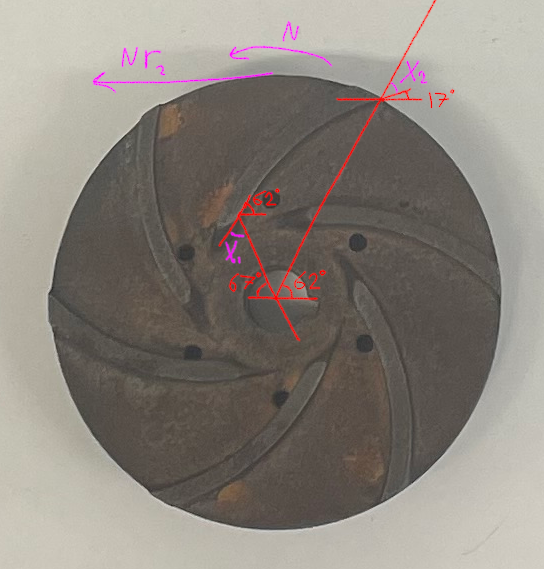
\includegraphics[width=0.6\textwidth]{impeller_annotations.png}
    \caption{Example image}
    \label{fig:impeller_annotations}
\end{figure}

And so angles of impeller blades to the radial direction are given by:
\begin{alignat}{2}
    \chi_1 &= 180 - 62 - 67 &= 51^\circ \notag \\
    \chi_2 &= 62 - 17 &= 45^\circ \notag
\end{alignat}

\subsection{Viscosiy measurements}

\begin{table}[H]
    \centering
    \begin{tabular}{|c|c|c|}
        \hline
        \textbf{Length} $(m)$ & \textbf{Time} (s) & \textbf{Density} ($kg/m^3$) \\
        \hline
        10 & 40.35 & 998.2 \\
        2 & 102.01 & 1170 \\
        \hline
    \end{tabular}
    \caption{Time taken for 10mL of fluid to travel a specific length at $18.3^\circ C.$}
    \label{tab:viscosity}
\end{table}

The ratio of dynamic viscosities of the fluids is given by the ratio of time to length.

\subsection{Compressor Data}

\begin{figure}[H]
    \centering
    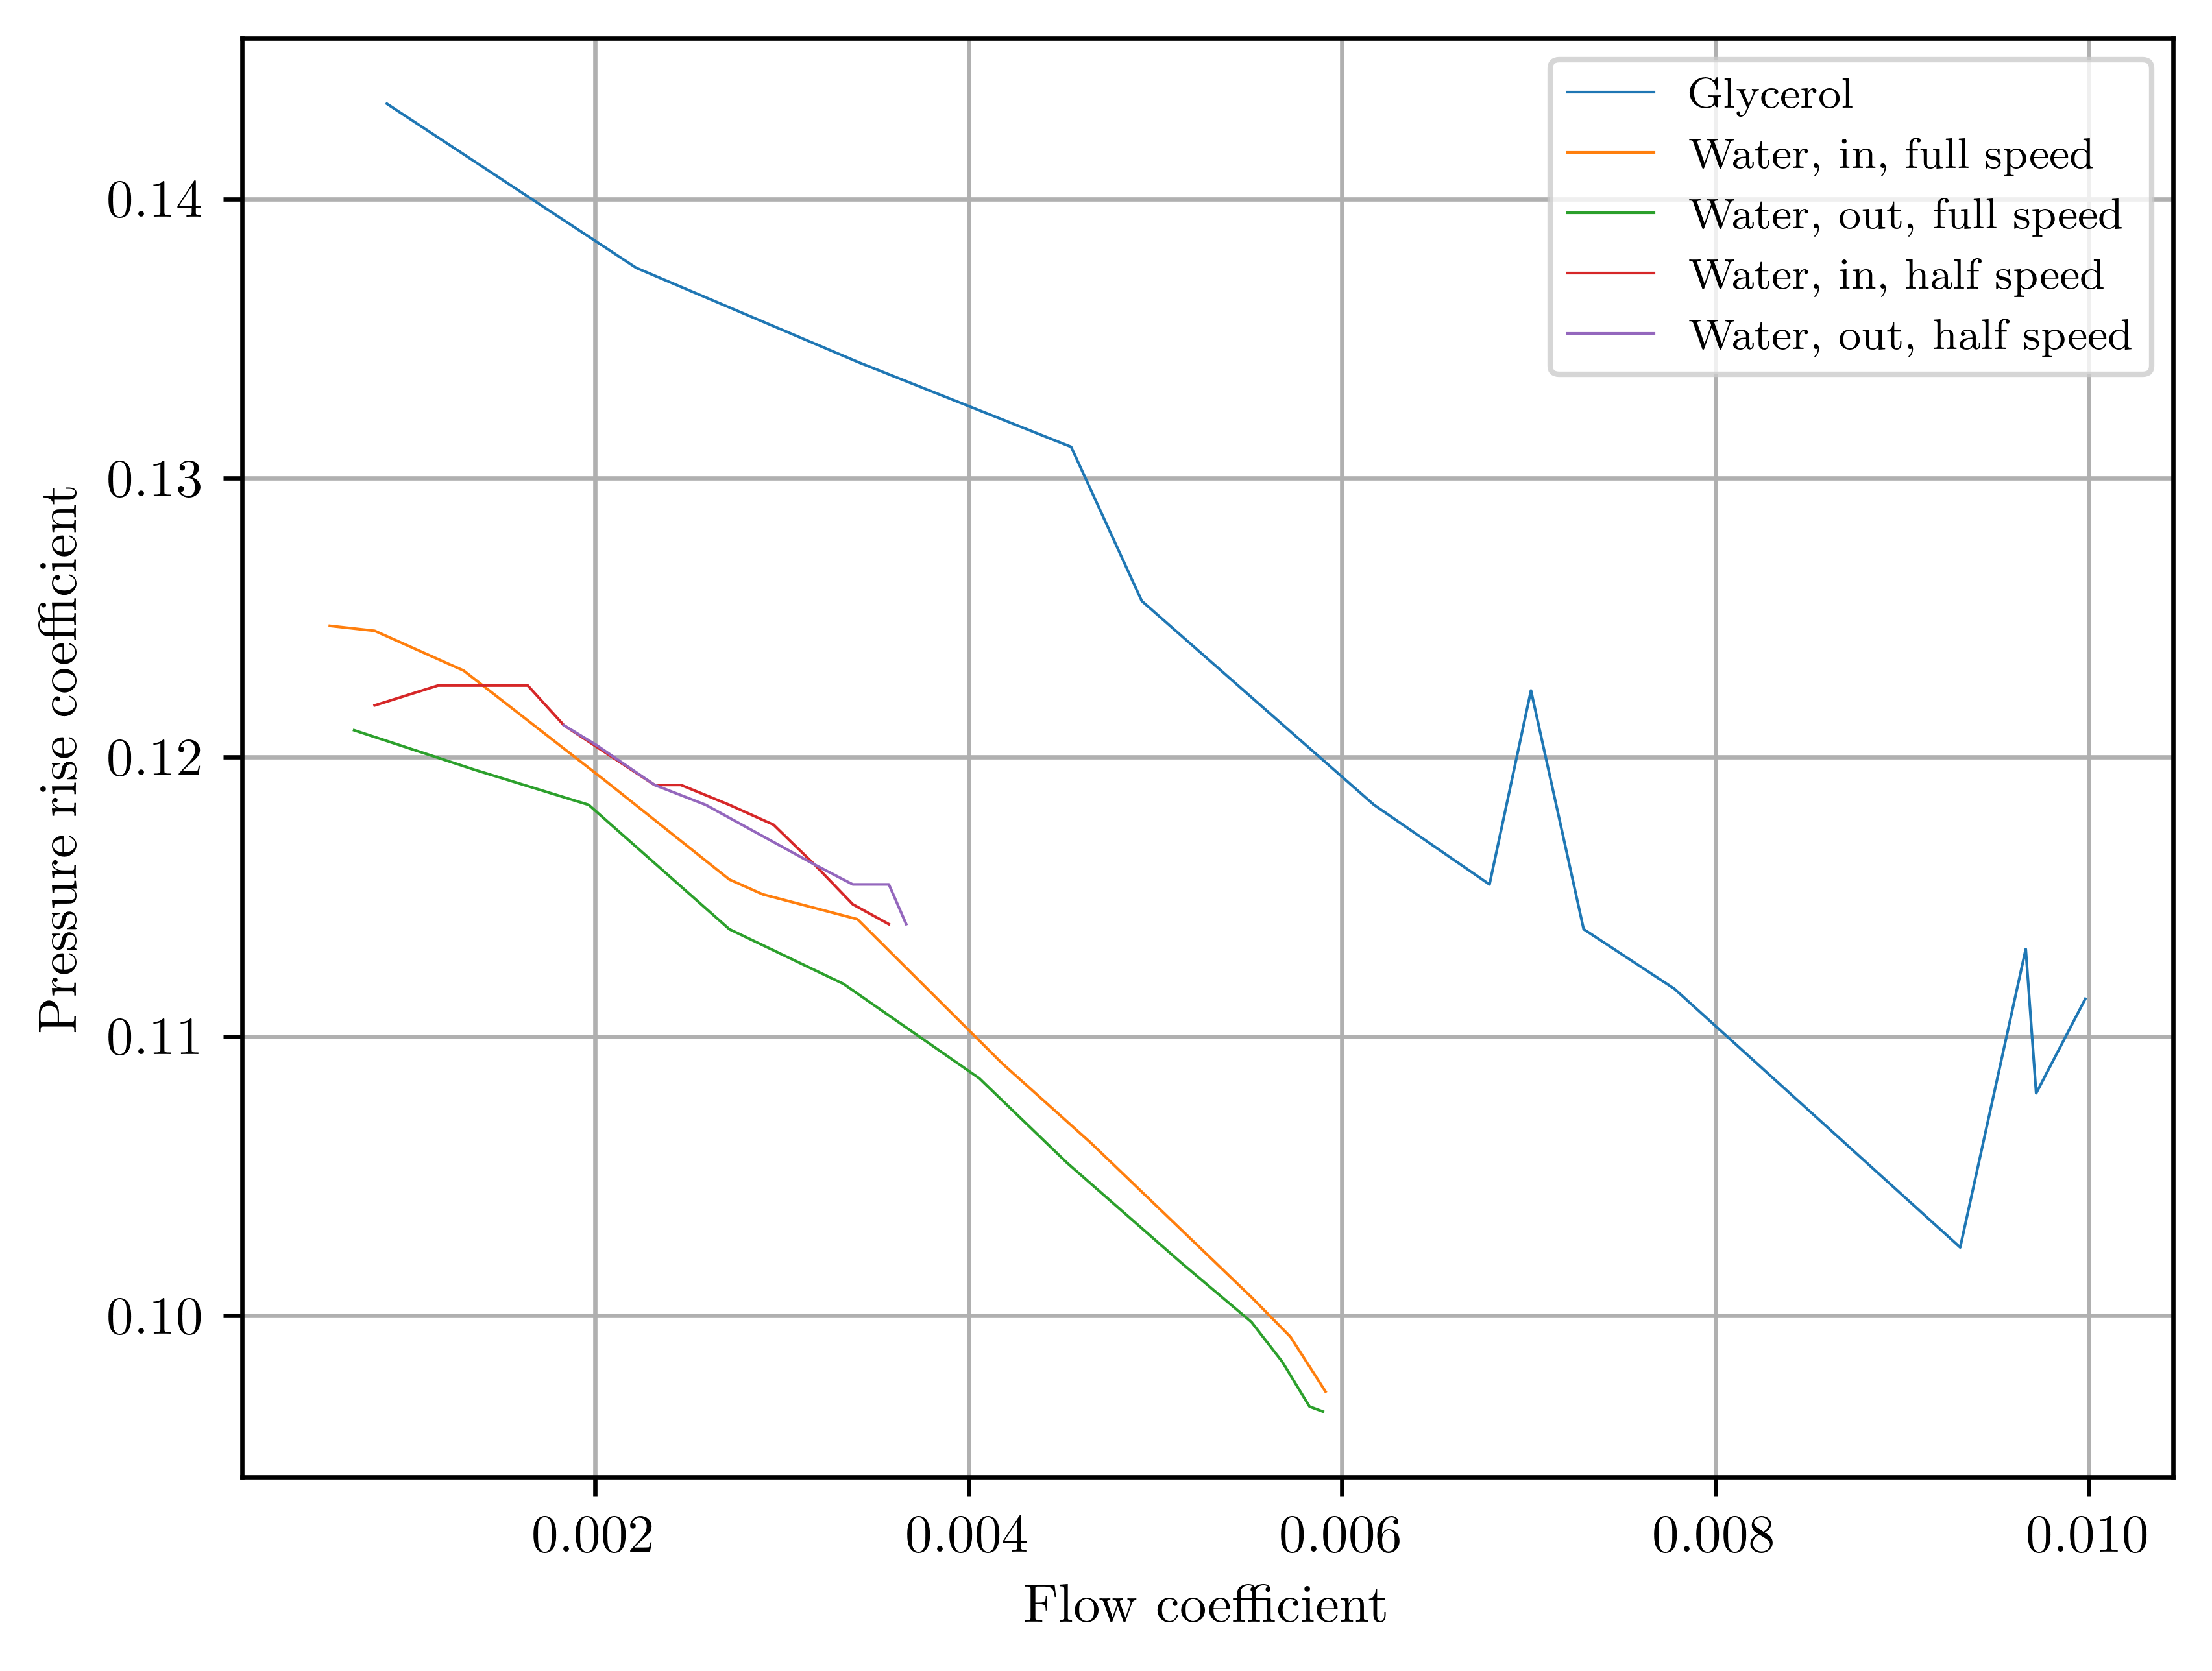
\includegraphics[width=0.99\textwidth]{compressor_non_dims.png}
    \caption{Non-dimensional pressure rise coefficient against non-dimensional flow coefficient various compressors conditions and setups.}
    \label{fig:compressor_non_dims}
\end{figure}

\section{Discussion}
% Analyze and interpret the results, discussing their significance and any observations or trends.

% Explain why throttling the water compressor at inlet and exit produce different cavitation
% results. Also explain why the pressure rise is similar when cavitation is not present.

why is pressure rise similar to when caviation is not present?

% Do the results agree with what you expect for:
%% Change of pressure rise with flow rate

The pressure coefficients for water at lower compressor speeds are higher than those at higher speeds, as expected.


%% Change of pressure rise with Reynolds number. Reference to figure 3 may be useful -
%% k/d is comparable to the roughness height of the blade surface divided by the channel span

%% Change in cavitation with rotor speed and throttle location? Sketch two velocity
%% triangles, one at a nominal design condition and when the flow coefficient is much lower.


%$ Can you explain the differences? Note that the two compressors do not give exactly the same
%% pressure rise-flow rate characteristics, and so care must be taken in comparing the effect of
%% Reynolds number.


% Suggest a reason why the venturi might not be suitable for measuring the flow rate of the
% glycerine solution.

\section{Conclusion}
% Summarize the main findings of the experiment and draw conclusions based on the results.

\end{document}
